\documentclass{beamer}
\usepackage{graphicx}
\usepackage{amssymb}
\usepackage{amsmath}
\usepackage{bm}
\graphicspath{{../resources/}}
\setbeamercovered{transparent}

\title{Slides for Summary States}
\author{Caleb Floyd and Tom Augspurger}
\date{\today}

\begin{document}

\frame{\titlepage}

% \section[Outline]{}
% \frame{\tableofcontents}

  % \begin{center}
  %   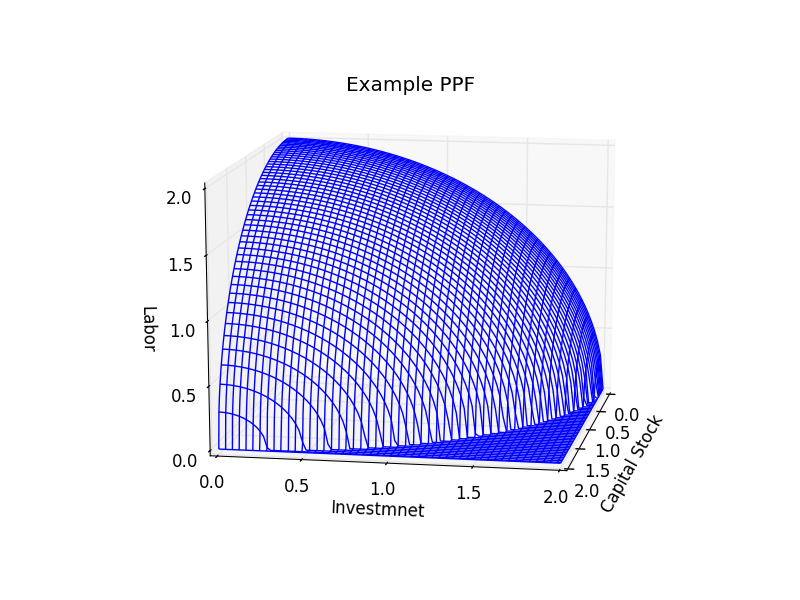
\includegraphics[scale=.31]{example_ppf_wire.png}
  %   \label{fig:ppf}
  % \end{center}

\begin{frame}[t]\frametitle{Growth in Patent Applications} 

  \begin{center}
      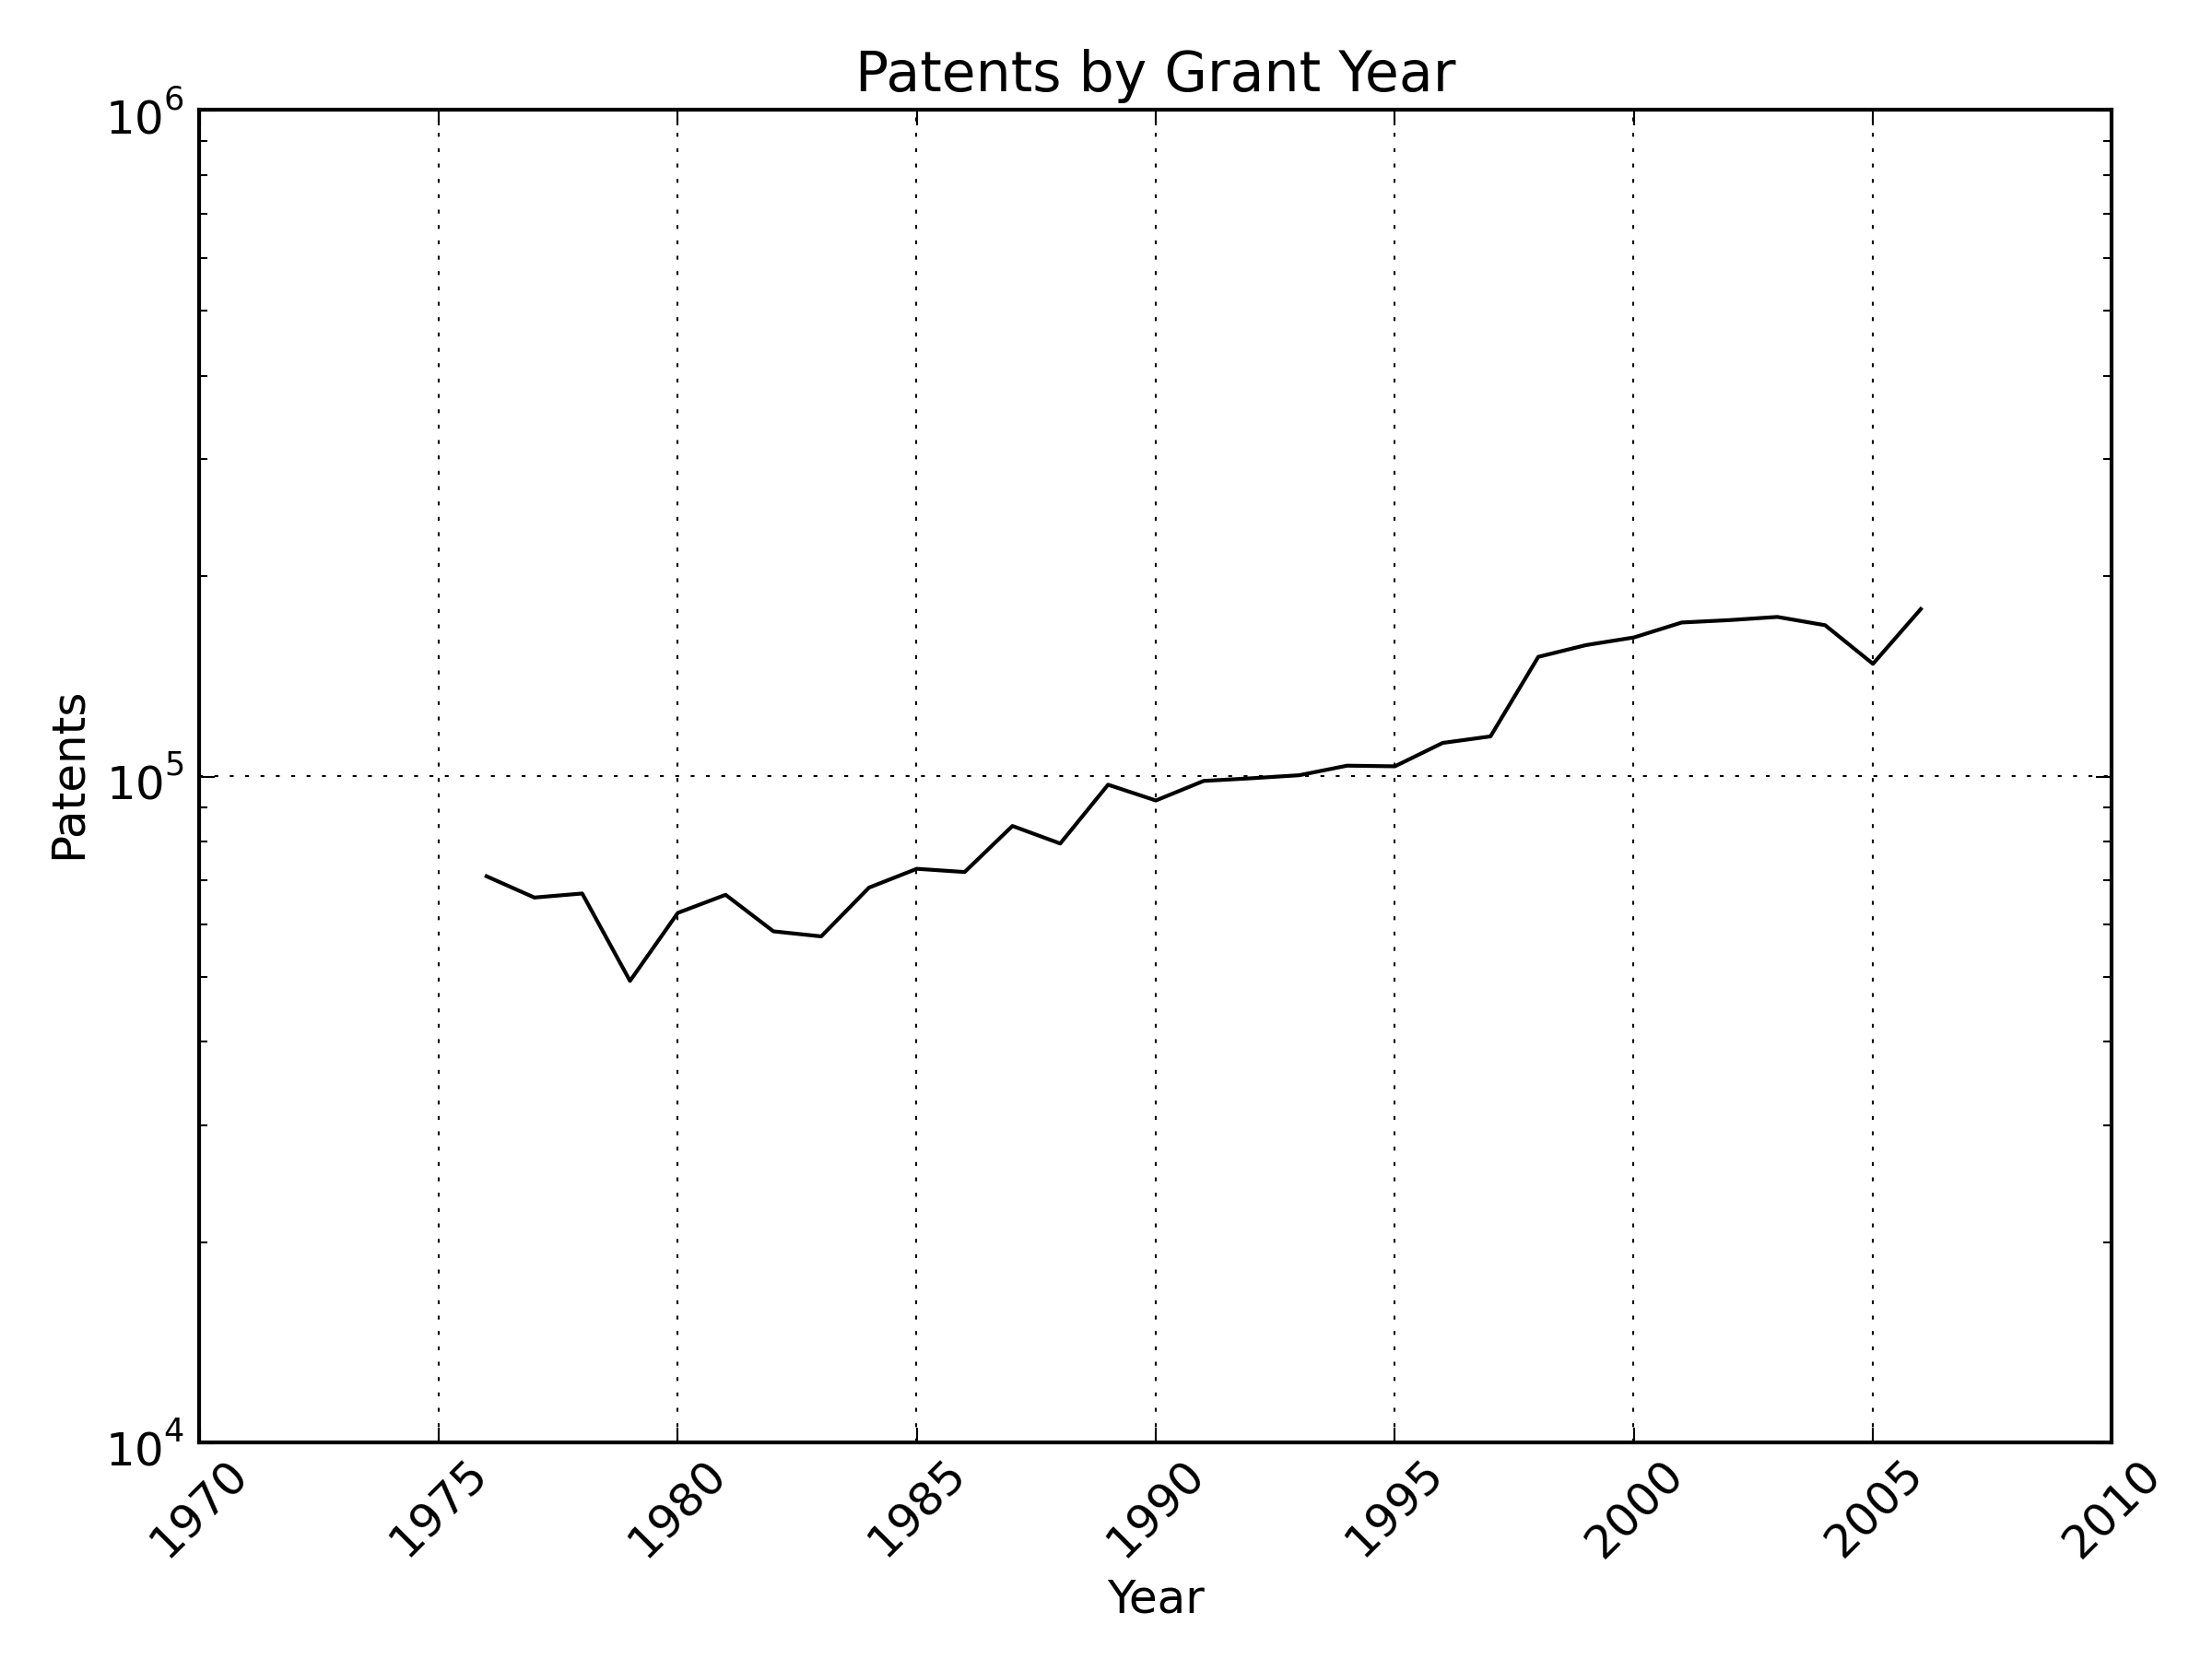
\includegraphics[scale=.5]{grant_year.png}
      \label{fig:grant_year}
  \end{center}
\end{frame}

\begin{frame}[t]\frametitle{Patents by Country} 

\begin{center}
  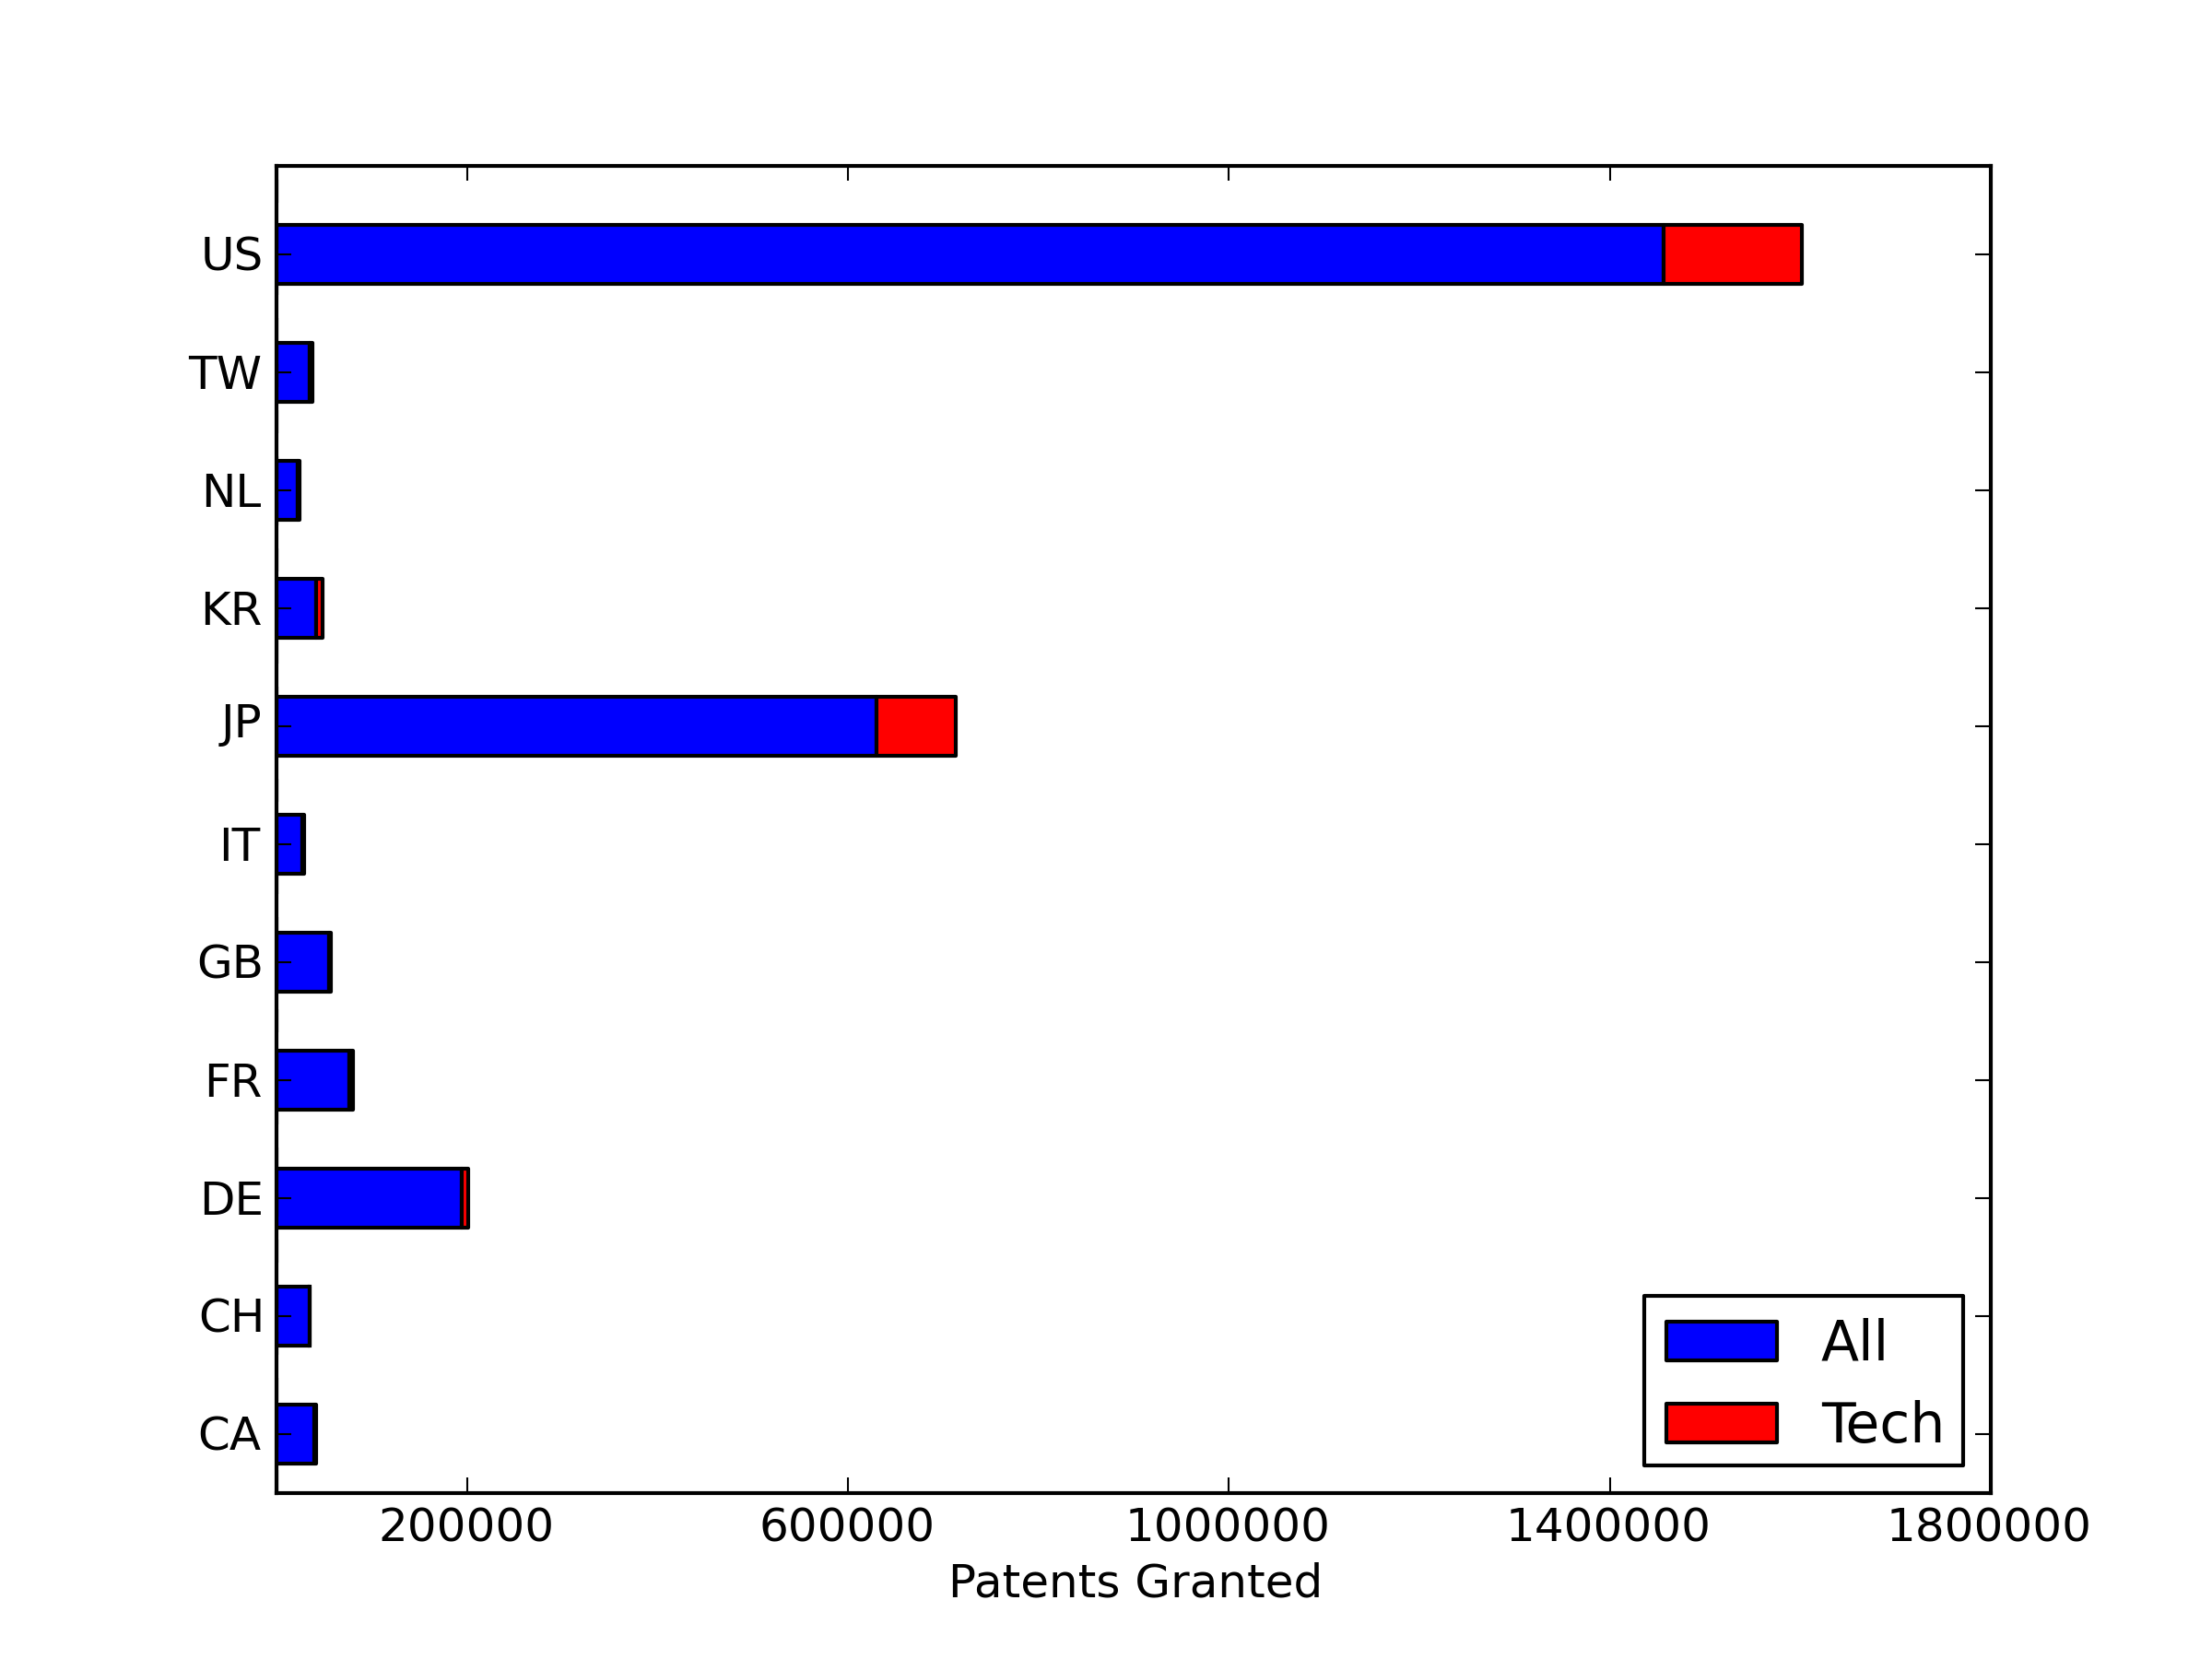
\includegraphics[scale=.5]{by_country.png}
  \label{fig:by_country}
\end{center}
\end{frame}

\begin{frame}[t]\frametitle{Patents by Country} 

\begin{center}
  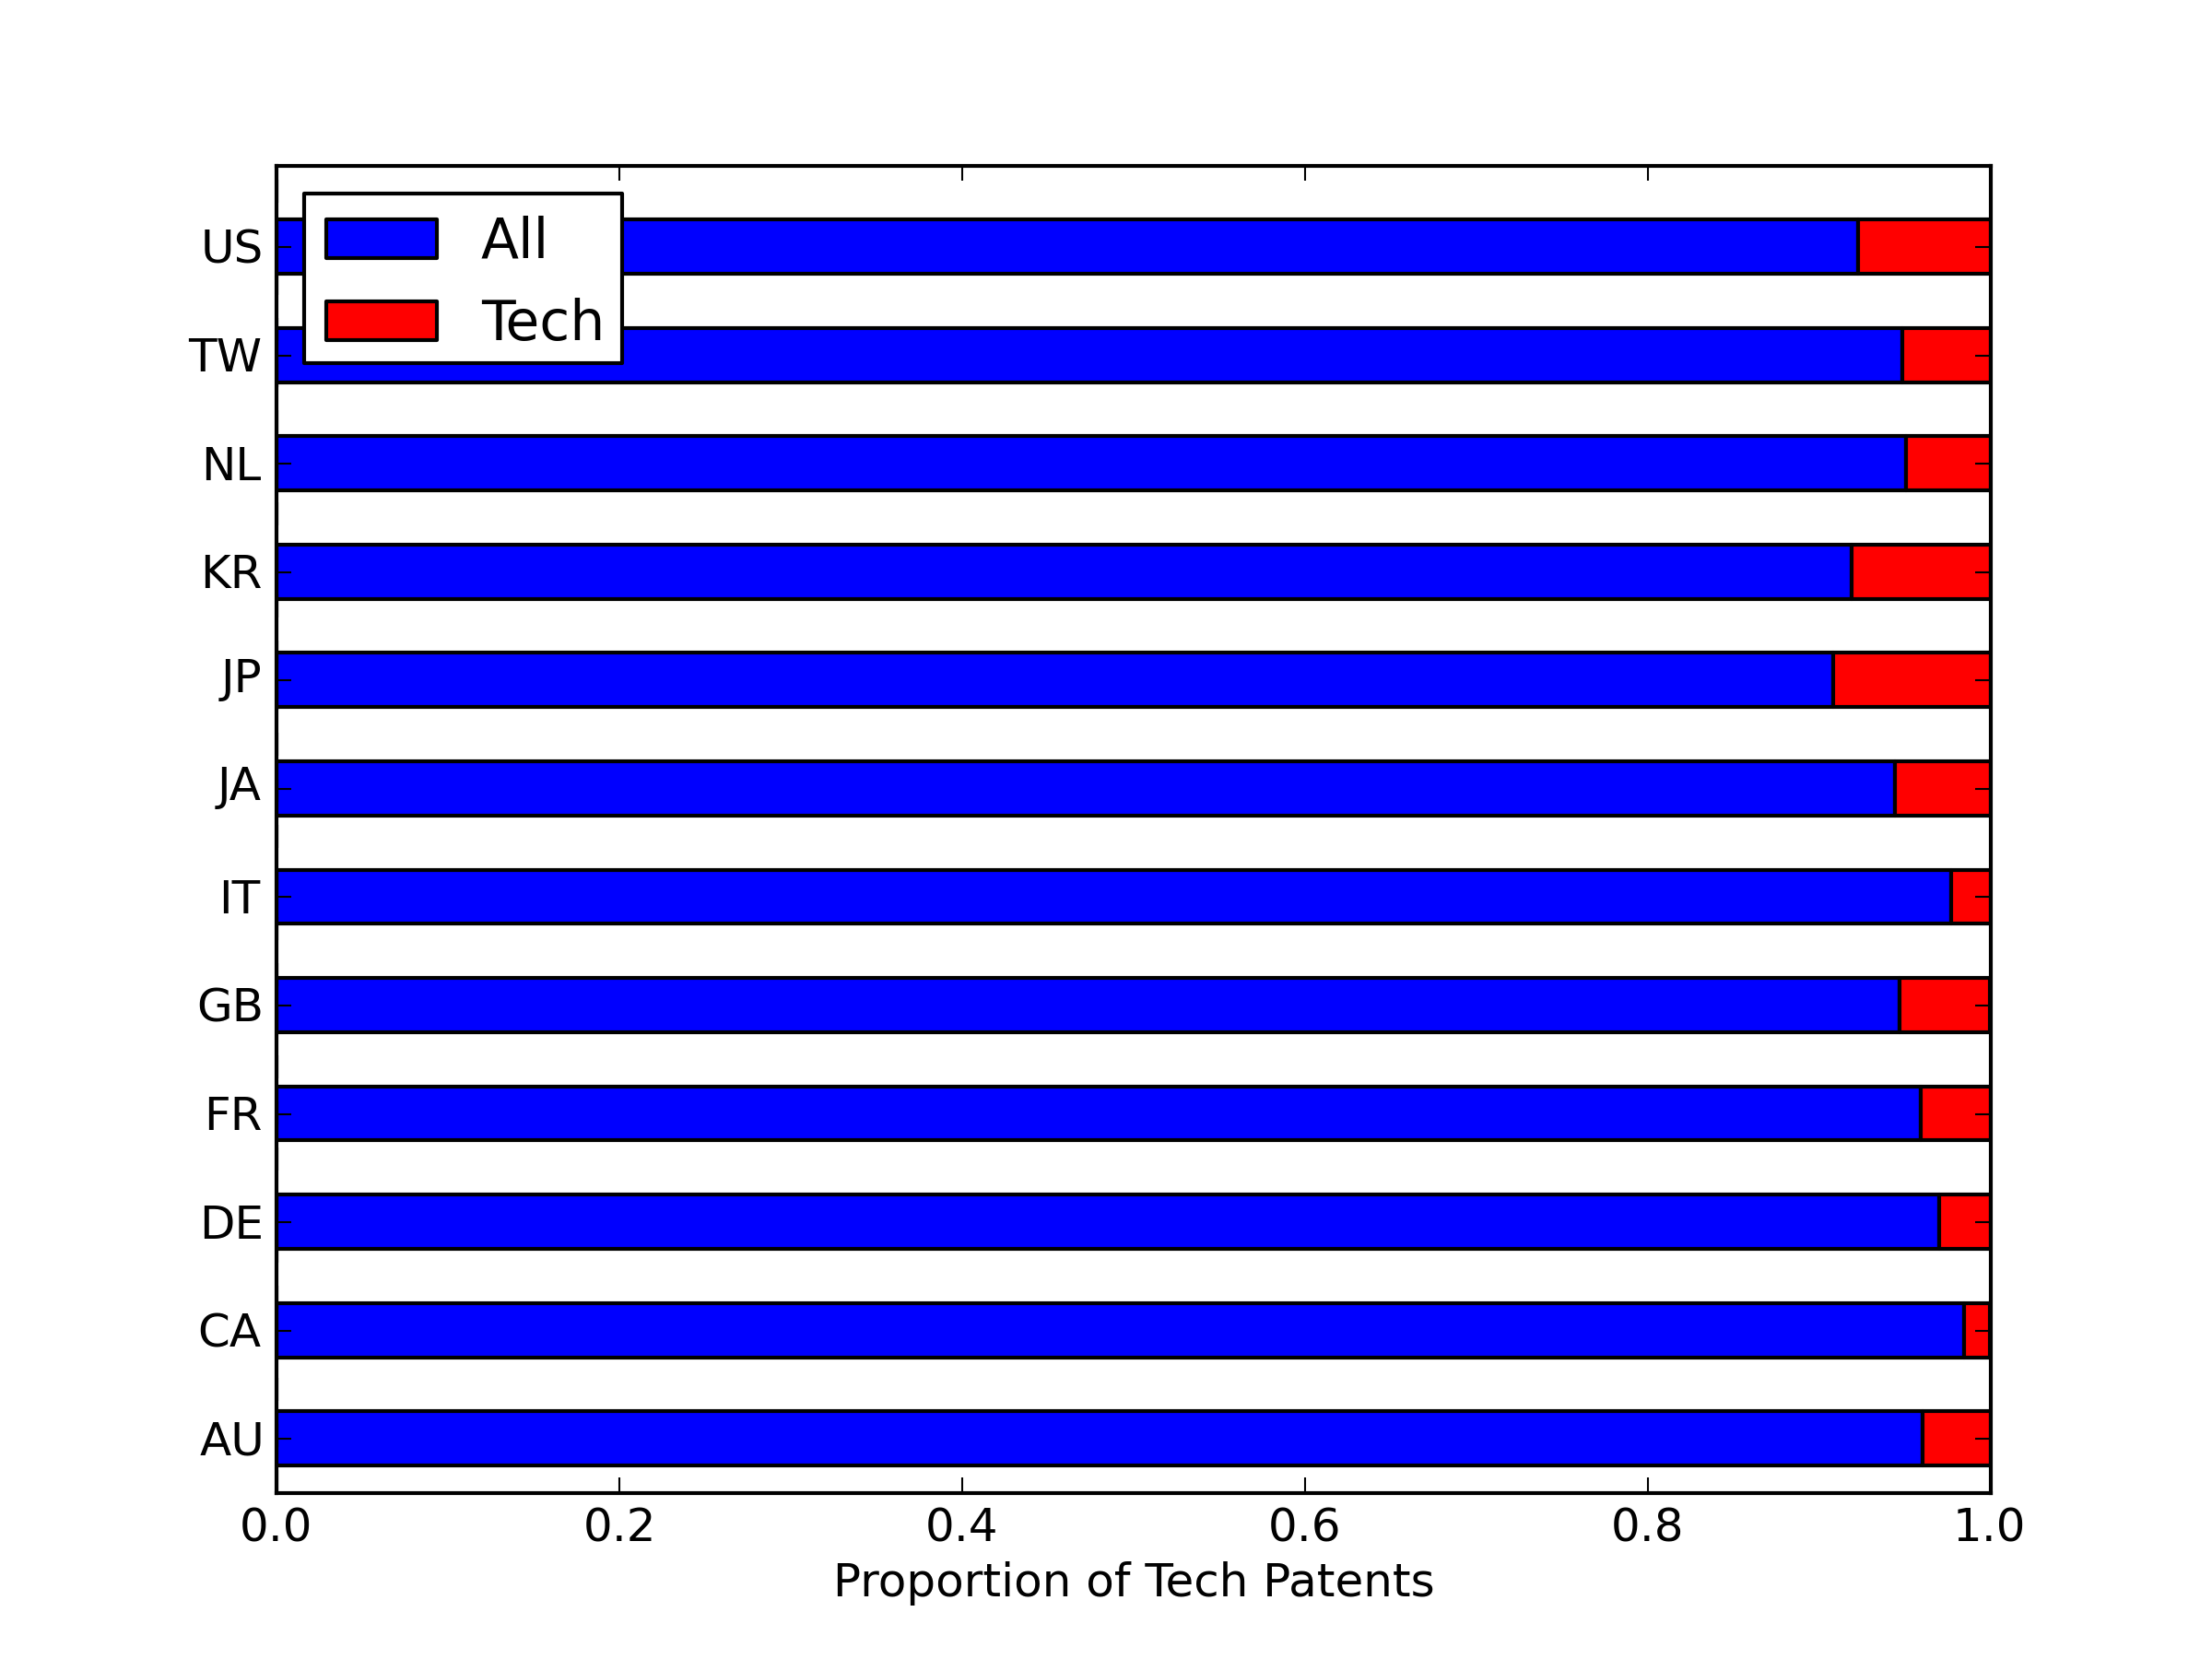
\includegraphics[scale=.5]{by_country_normalized.png}
  \label{fig:by_country_normalized}
\end{center}
\end{frame}

\begin{frame}[t]\frametitle{Most Cited Patent} 
  \begin{itemize}
    \item<+-> February 2, 1988: Patent No. 4,723,129.
    \item<+-> Bubble jet recording method and apparatus in which a heating element generates bubbles in a liquid flow path to project droplets 
  \end{itemize}
\end{frame}


\begin{frame}[t]\frametitle{Most Cited Patent} 
  \begin{itemize}
    \item February 2, 1988: Patent No. 4,723,129.
    \item Bubble jet recording method and apparatus in which a heating element generates bubbles in a liquid flow path to project droplets 
    \item Canon Ink Jet printers.
  \end{itemize}
\end{frame}


\end{document}
